% Split-fill plot marks used as workflow checkpoints.
\documentclass[border=2pt]{standalone}
\usepackage{tikz}
\usetikzlibrary{arrows.meta,plotmarks,positioning}

\begin{document}
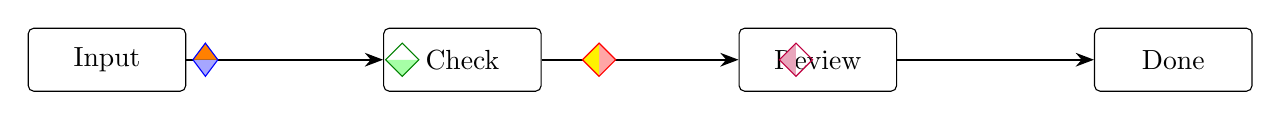
\begin{tikzpicture}[
  node distance=2.5cm,
  stage/.style={draw,rounded corners=2pt,minimum width=2cm,minimum height=8mm},
  flow/.style={-Stealth,thick}
]
  \node[stage] (input) {Input};
  \node[stage,right=of input] (check) {Check};
  \node[stage,right=of check] (review) {Review};
  \node[stage,right=of review] (done) {Done};
  \draw[flow] (input) -- (check);
  \draw[flow] (check) -- (review);
  \draw[flow] (review) -- (done);
  \draw[blue,fill=blue!35,mark color=orange,mark size=6pt]
    plot[mark=halfdiamond*] coordinates {(1.25,0)};
  \draw[green!50!black,fill=green!35,mark color=white,mark size=6pt]
    plot[mark=halfsquare*] coordinates {(3.75,0)};
  \draw[red,fill=red!35,mark color=yellow,mark size=6pt]
    plot[mark=halfsquare right*] coordinates {(6.25,0)};
  \draw[purple,fill=purple!35,mark color=none,mark size=6pt]
    plot[mark=halfsquare left*] coordinates {(8.75,0)};
\end{tikzpicture}
\end{document}
